\chapter*{Breve panoramica sulla libreria CFLIB - Python}
\addcontentsline{toc}{chapter}{Breve panoramica sulla libreria CFLIB - Python}
\section*{Riferimenti di Posizione}
\addcontentsline{toc}{section}{Riferimenti di Posizione}

Questa libreria è stata appositamente sviluppata da Bitcraze e contiene tutte le funzioni necessarie per comunicare da/verso il Drone. Essendo open-source al suo sviluppo può contribuire chiunque e c’è molta disponibilità di materiale sul web. 
\\
La libreria contiene svariate classi grazie a cui si possono inviare comandi al Drone, di seguito a titolo di esempio e soltanto per fornire un’idea di come queste funzioni sono implementate, mostreremo alcune delle funzioni e andremo ad analizzarle passando dal vedere come queste sono disponibili “ad alto livello” e guardando come si implementano “a basso livello” fino alle funzioni che implementano l’invio dei pacchetti CRTP spiegati in precedenza. 
\\
Un esempio è la classe \verb Commander  che consente di inviare al Drone riferimenti di posizione da inseguire e che è la stessa utilizzata nel nostro codice. Ne vediamo un estratto in figura ~\ref{fig:funzioniAltoLivello}.
\\
In realtà per essere più precisi specifichiamo che nel codice utilizzeremo anche una variante della classe \verb Commander  e che si chiama \verb MotionCommander  . La particolarità di quest'ultima è che consente di effettuare la procedura di decollo in modo "automatico" una volta creato il relativo oggetto Dorne. Avremo dunque nel nostro codice un oggetto per ognuna di queste due classi ma utilizzeremo questa variante soltanto per effettuare il decollo mentre per l'intera parte rimanente ci avvaleremo della classe \verb Commander . 
\begin{figure}[h]
    \centering
    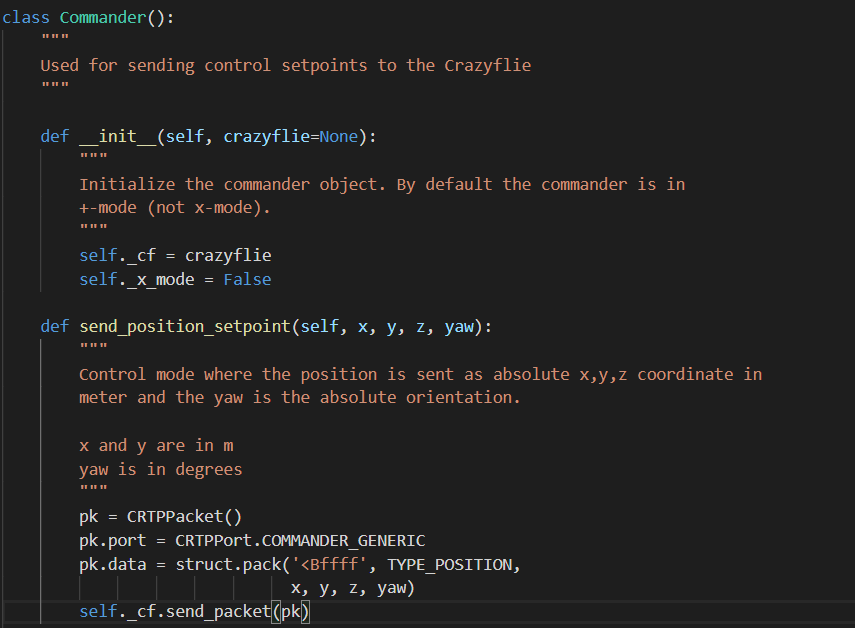
\includegraphics[width=0.8 \textwidth]{Relazione/Immagini/funzioniAltoLivello.PNG}
    \caption{Classe Commander}
    \label{fig:funzioniAltoLivello}
\end{figure}

\\
Al loro interno queste funzioni consentono di costruire i pacchetti CRTP a partire dai valori dei riferimenti desiderati.
L'invio del pacchetto è fatto in accordo con quanto previsto dal protocllo CRTP utilizzando la send\_packet riportata in figura ~\ref{fig:sendPacketPyton}. 
\\
\begin{figure}[h]
    \centering
    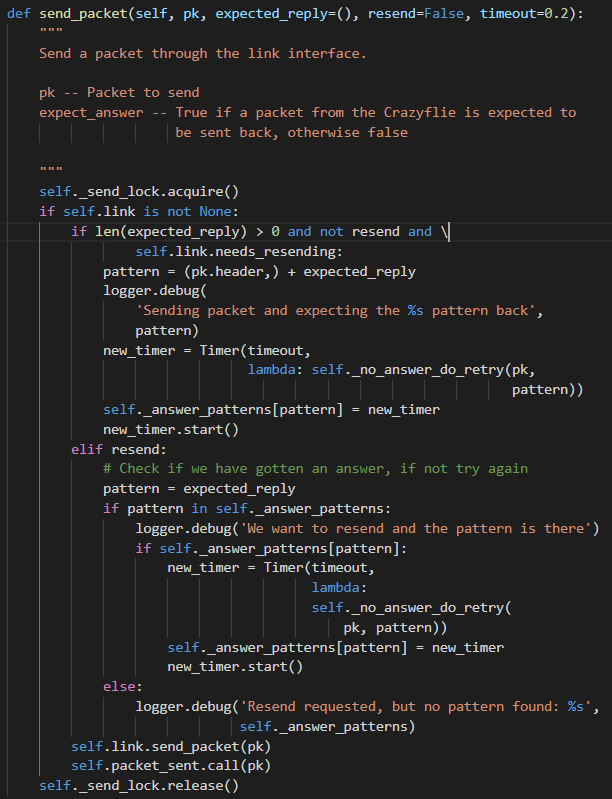
\includegraphics[width=0.8 \textwidth]{Relazione/Immagini/sendPacketPyton.png}
    \caption{send\_packet - Chiamata all'interno della send\_setpoint responsabile del solo handshake iniziale}
    \label{fig:sendPacketPyton}
\end{figure}
\\
A sua volta questa funzione ricorre alle funzioni proprie del driver della Crazyradio. In figura ~\ref{fig:sendPacket} riportiamo la send\_packet che di fatto consente alla Crazyradio di inviare il pacchetto CRTP (notiamo come questa, essendo parte del firmware è scritta in C). 
\\
\begin{figure}[h]
    \centering
    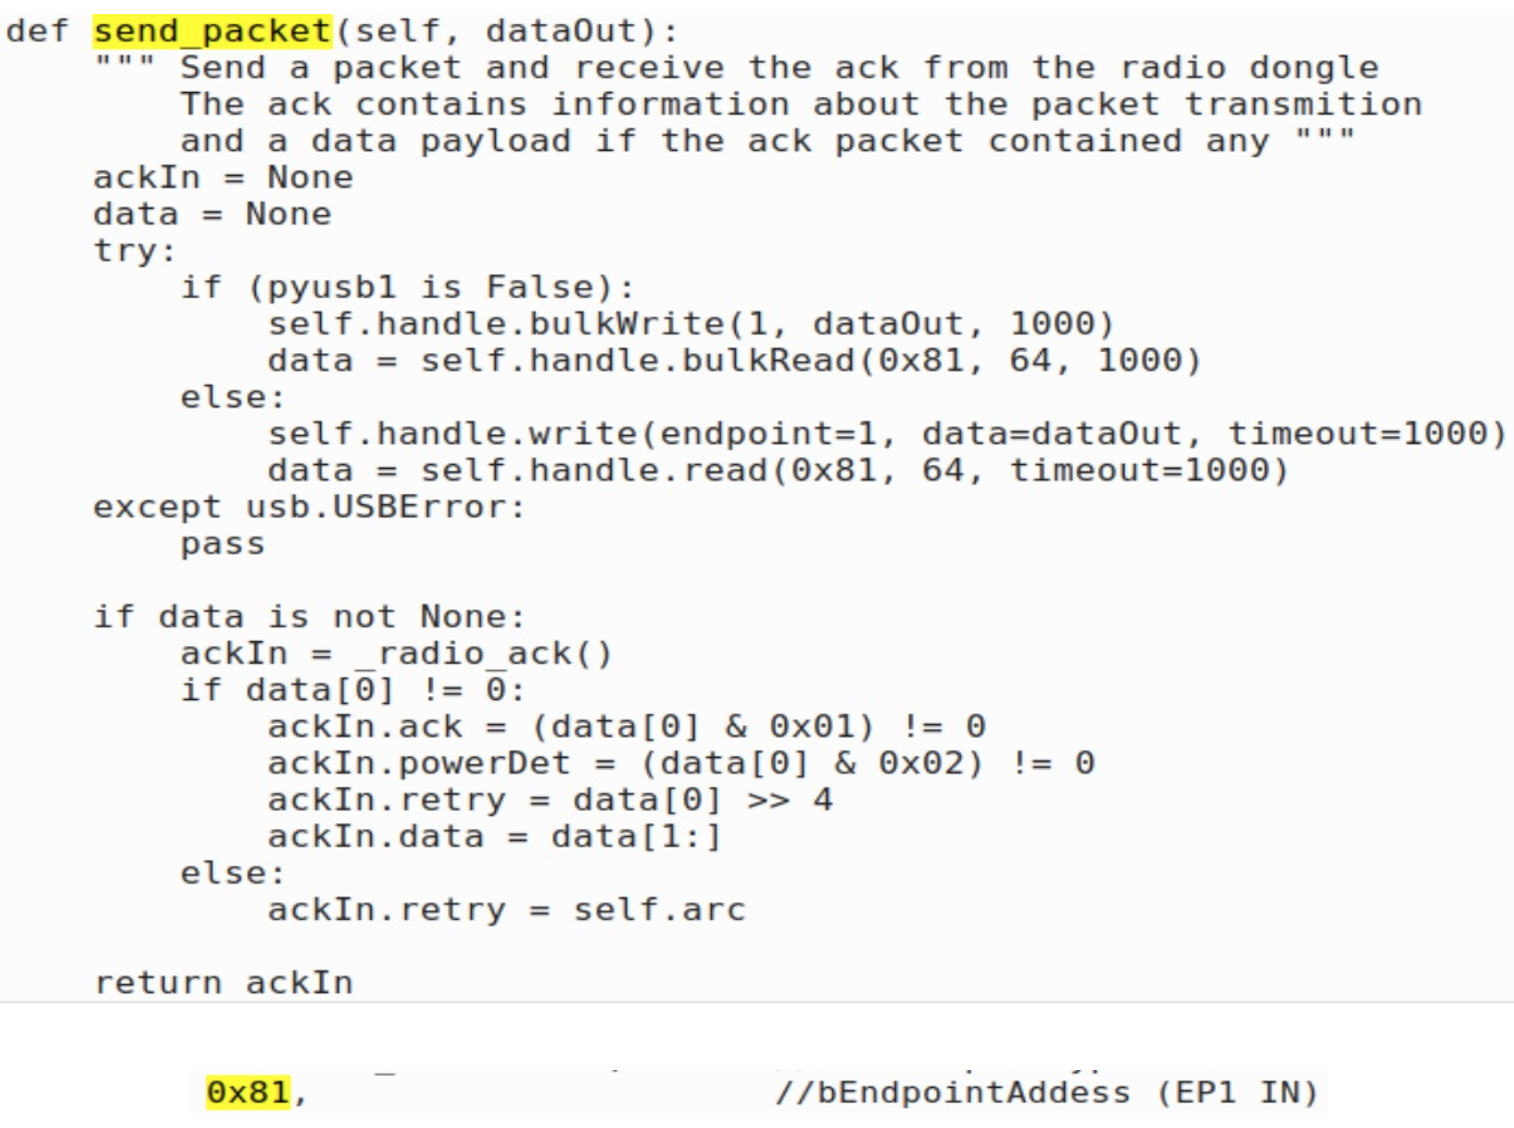
\includegraphics[width=0.8 \textwidth]{Relazione/Immagini/sendPacket.png}
    \caption{send\_packet - Tramite la bulkWrite invia dataOut per poi attendere quanto ricevuto dal Drone e metterlo in data}
    \label{fig:sendPacket}
\end{figure}
\\
\section*{Aggiornamento filtro di Kalman}
\addcontentsline{toc}{section}{Aggiornamento filtro di Kalman}
\\
Per inviare le misure di posizione al filtro di Kalman utilizziamo la funzione \verb send_extpos  che riportiamo in figura ~\ref{fig:sendextpos}.

\begin{figure}[h]
    \centering
    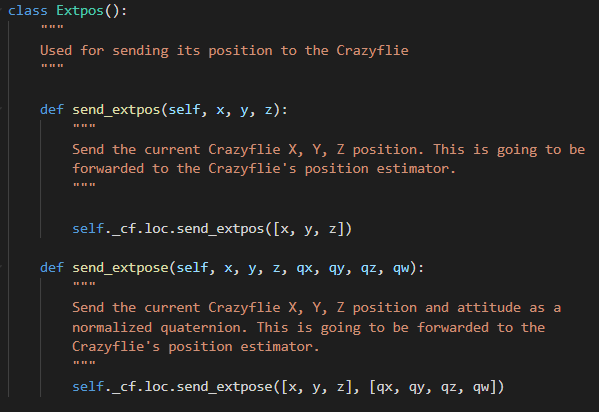
\includegraphics[width=0.8 \textwidth]{Relazione/Immagini/sendextpos.png}
    \caption{In figura sono riportate sia la send\_extpos, utilizzata per l'invio della sola posizione, che la send\_extpose, utilizzata per l'invio di posizione e orientazione}
    \label{fig:sendextpos}
\end{figure}

\\
\\
Per quanto riguarda la gestione dei messaggi nel caso di ricezione (da parte del Drone) di informazioni di posizione da utilizzare per l’aggiornamento del filtro di Kalman, ricordando quanto detto precedentemente, si riporta nelle figure che vanno dalla ~\ref{fig:externalPositionRiassunto} alla ~\ref{fig:genericPositionHandler} il “percorso” (in termini di funzioni della libreria) seguito dal pacchetto una volta ricevuto e “spacchettato” dal Crazyflie.

\begin{figure}[h]
    \centering
    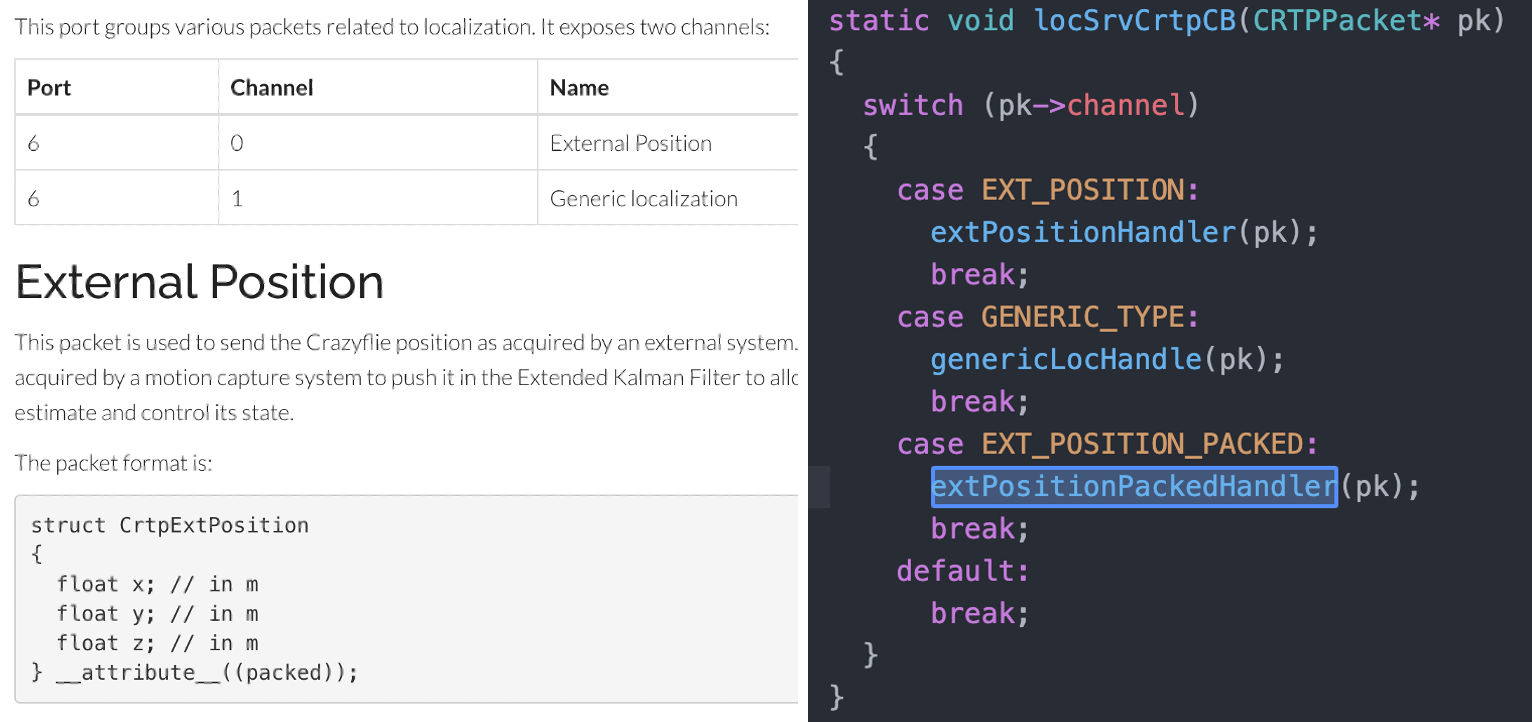
\includegraphics[width=0.8 \textwidth]{Relazione/Immagini/externalPositionRiassunto.png}
    \caption{a seconda del canale scritto nel pacchetto l’informazione viene gestita da funzioni diverse che, a seconda del caso, operano secondo quanto stabilito dal protocollo CRTP}
    \label{fig:externalPositionRiassunto}
\end{figure}
\\
\begin{figure}[h]
    \centering
    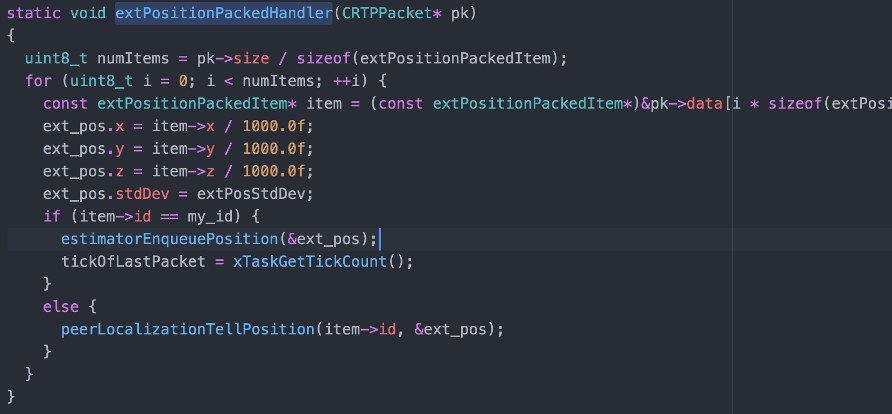
\includegraphics[width=0.8 \textwidth]{Relazione/Immagini/extPositionPackedHandler.png}
    \caption{Qui notiamo l’utilizzo dell’informazione della sola posizione per assegnarla al valore attuale di posizione del Drone e la messa in coda tra i dati da utilizzare per il filtro di Kalman.}
    \label{fig:extPositionPackedHandler}
\end{figure}
\\
\begin{figure}[h]
    \centering
    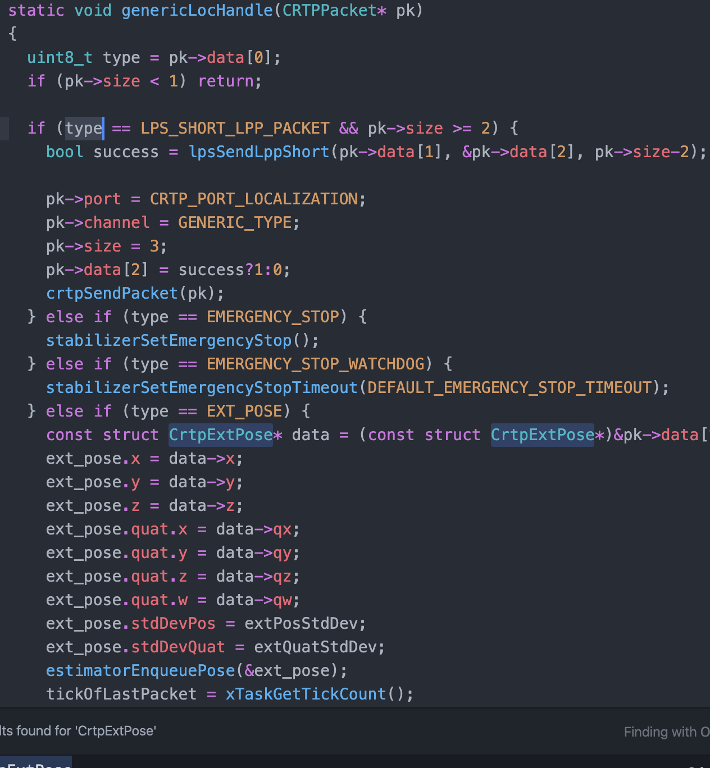
\includegraphics[width=0.8 \textwidth]{Relazione/Immagini/genericPositionHandler.png}
    
    \caption{Qui vediamo invece come viene gestita l’informazione quando riceviamo, oltre alla posizione, anche l’orientazione. 
Il ramo di codice di interesse è quello relativo a “type == EXT\_POSE” (in cui EXT\_POSE vale 8).
}
    \label{fig:genericPositionHandler}
\end{figure}
\\
In entrambi i casi, sia che si passi dalla \verb genericPositionHandler  sia che si passi  dalla \\ \verb extPositionHandler 
, una volta inseriti nella coda i dati vengono elaborati come in figura ~\ref{fig:kalmanCoreUpdate}. 
\\
\begin{figure}[h]
    \centering
    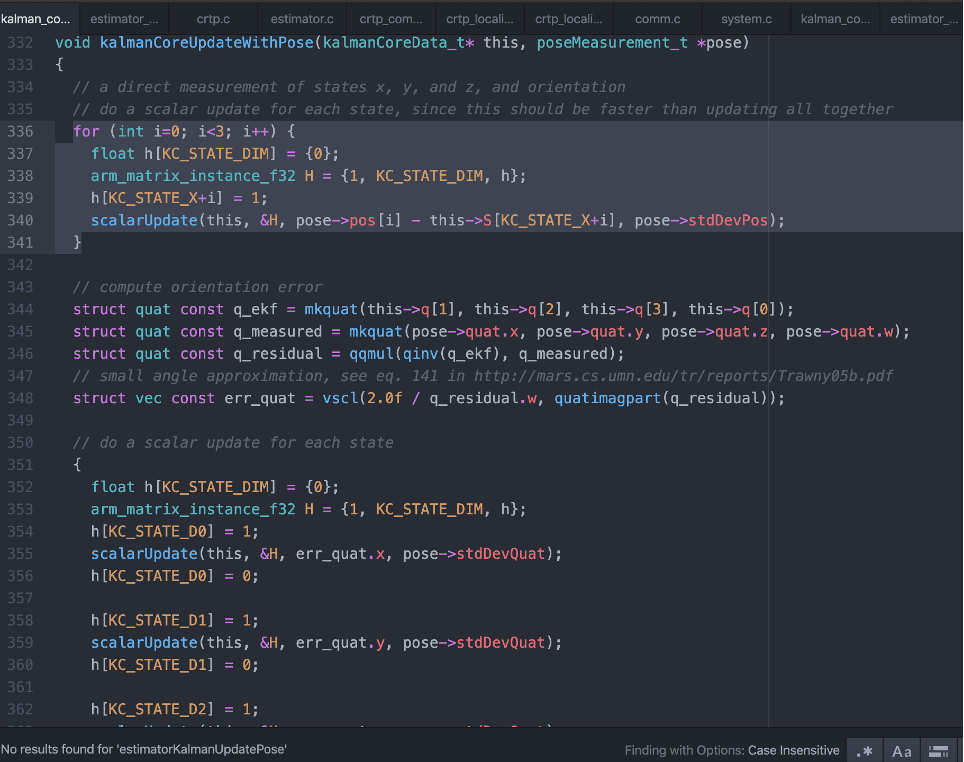
\includegraphics[width=0.8 \textwidth]{Relazione/Immagini/kalmanCoreUpdate.png}
    \caption{}
    \label{fig:kalmanCoreUpdate}
\end{figure}
